% !TEX ROOT = ersti.tex
\section*{Ansprechpartner im Studium}

Nicht nur am Anfang eures Studiums, sondern auch mitten drin können kleinere und größere Fragen und Probleme auftreten. Damit ihr mit diesen Problemen nicht alleine da steht, gibt es mehrere Personen, die euch bei diesen helfen können. Erste Ansprechpartnerin in allen Dingen ist natürlich die Fachschaft. Falls wir euch dann nicht weiter helfen können, gibt es an jeder Fakultät noch weitere Ansprechpartnerinnen.

\newcommand{\proffoto}[2]{
    \centering
    \includegraphics[width=3.5cm]{#1}\\
    #2
    \vspace{4mm}
}

\begin{figure}[b]
	\vspace*{4mm}
    \begin{subfigure}{.50\linewidth}
        \ifdefined\dekanphysikfoto
        \proffoto{\dekanphysikfoto}{\dekanphysiklang\\[-1ex]{\scriptsize Dekan Physik}}
        \fi
    \end{subfigure}
    \begin{subfigure}{.42\linewidth}
    	\vspace{-8mm} %Feinjustierung

        \ifdefined\dekanmathefoto
        \proffoto{\dekanmathefoto}{\dekanmathelang\\[-1ex]{\scriptsize Dekan Mathe \& Info}}
        \fi
    \end{subfigure}
\end{figure}

\begin{figure*}
    \centering
    \begin{subfigure}{.3\linewidth}
        \ifdefined\studiendekanphysikfoto
        \proffoto{\studiendekanphysikfoto}{\studiendekanphysik\\[-1ex]{\scriptsize Studiendekan Physik}}
        \fi
    \end{subfigure}
    \begin{subfigure}{.3\linewidth}
        \ifdefined\studiendekanmathefoto
        \proffoto{\studiendekanmathefoto}{\studiendekanmathe\\[-1ex]{\scriptsize ~ Studiendekan Mathe}}
        \fi
    \end{subfigure}
    \begin{subfigure}{.3\linewidth}
        \ifdefined\studiendekaninformatikfoto
        \proffoto{\studiendekaninformatikfoto}{\studiendekaninformatik\\[-1ex]{\scriptsize ~ Studiendekan Info}}
        \fi
    \end{subfigure}
\end{figure*}


\begin{description}
%\sidebar{
%    \chaptersidebarpushdown
%    \ifdefined\dekanphysikfoto
%    \proffoto{\dekanphysikfoto}{\dekanphysiklang\\[-1ex]{\scriptsize Dekan Physik}}
%    \fi
%
%    \ifdefined\dekanmathefoto
%   \proffoto{\dekanmathefoto}{\dekanmathelang\\[-1ex]{\scriptsize Dekan Mathe \& Info}}
%    \fi
%
%    \ifdefined\studiendekaninformatikfoto
%    \proffoto{\studiendekaninformatikfoto}{\studiendekaninformatik\\[-1ex]{\scriptsize Studiendekan Info}}
%    \fi
%
%    \ifdefined\studiendekanphysikfoto
%    \proffoto{\studiendekanphysikfoto}{\studiendekanphysik\\[-1ex]{\scriptsize Studiendekan Physik}}
%    \fi
%
%   \vspace*{1.8cm}
%
%    \ifdefined\studiendekanmathefoto
%    \proffoto{\studiendekanmathefoto}{\studiendekanmathe\\[-1ex]{\scriptsize Studiendekan Mathe}}
%    \fi
%\iffalse
%    \ifdefined\prodekanmathefoto
%   \proffoto{\prodekanmathefoto}{\prodekanmathe\\[-1ex]{\scriptsize Prodekan Mathe \& Info}}
%    \fi
%
%    \ifdefined\prodekanphysikfotoA
%    \proffoto{\prodekanphysikfotoA}{\prodekanphysikA\\[-1ex]{\scriptsize Prodekan Physik}}
%    \fi
%
%    \ifdefined\prodekanphysikfotoB
%    \proffoto{\prodekanphysikfotoB}{\prodekanphysikB\\[-1ex]{\scriptsize Prodekan Physik}}
%    \fi
%\fi
%    % Rest weiter unten weil die Physik zwei Prodekane hat
%    % und damit nicht mehr alles in die Spalten passt
%}

\item[Die Dekanin] ist sozusagen Chefin der Fakultät und leitet diese. Sie wird für vier Jahre gewählt. In der Mathe \& Informatik ist \dekanmathelang\ Dekan, in der Physik \dekanphysiklang .

\item[Die Prodekanin] ist Vertreterin der Dekanin und unterstützt diese in ihren Aufgaben. In der Mathe \& Informatik ist \prodekanmathe\ Prodekan, in der Physik \prodekanphysik .\\[2em]

\item[Das Dekanat] ist das Sekretariat der Fakultät. Hier kann euch geholfen werden, wenn ihr nicht wisst, an wen ihr euch genau wenden sollt\footnote{In der Mathe \& Info: Tel.  \dekanatmathetelefon , in der Physik: Tel. \dekanatphysiktelefon}.

\item[Die Studiendekanin] ist Vorsitzende der Studienkommission. Diese ist für alle Fragen der Lehre zuständig und auch die erste Adresse bei Fragen und Problemen. In der Mathe ist \studiendekanmathe\ Studiendekan, in der Informatik \studiendekaninformatik , in der Physik \studiendekanphysik .

\item[Die Studienberaterinnen] beantworten Fragen zur persönlichen Studienplanung, zur Orientierung und zum Studium allgemeinen. So zum Beispiel \studienberatungmathe\ in der Mathe, \studienberatunginformatik\ in der Informatik und \studienberatungphysik\ in der Physik.

\item[Deine Fachschaft] vertritt die Interessen der Studierenden in den Fakultätsgremien und ist diskrete Ansprechpartnerin bei Problemen mit einer Dozentin oder Fragen zur Prüfungsordnung. \\\fsraum; \url{fachschaft@mathphys.info}

\item[Das Prüfungssekretariat] ist zuständig für Prüfungsfragen aller Art. Ob es jetzt um die Anrechnung von Modulen anderer Fakultäten, die Anmeldung von Bachelorarbeiten oder sonstige Fragen rund um die Prüfungsordnung geht, im Prüfungssekretariat sitzen kompetente Menschen, die dir weiterhelfen. In der Informatik ist das \pruefsekinfo, in der Mathe \pruefsekmathe, in der Physik \pruefsekphysik.

\item[Der Prüfungsausschuss] hilft da, wo das Prüfungssekretariat nicht weiter weiß. Er ist die letzte Instanz in Fragen der Prüfungsordnung. Meist hat man aber nur mit dem Vorsitz zu tun. In der Physik ist das \pruefausschussvorsitzphysik, in der Mathe \pruefausschussvorsitzmathe, in der Informatik \pruefausschussvorsitzinformatik.

\item[BAföG-Beauftragte] Spätestens zu Beginn des 5. Semesters braucht ihr einen Leistungsnachweis, dass ihr die bei geordnetem Verlauf der Ausbildung bis zum Ende des 4. Fachsemesters üblichen Leistungen erbracht habt. Dies bestätigt euch in der Mathe \bafogmathe , in der Informatik \bafoginformatik\ und in der Physik \bafogphysik .

\item[Lehramt] Alle Fragen, die das Lehramt betreffen, können euch im Zentrum für Lehrerbildung beantwortet werden: ZLB, Akademiestraße 3, Zimmer 237

\item[Gleichstellungskommissionen] setzen sich für die Chancengleichheit von Frauen und Männern ein und informieren über gesetzliche Regelungen. Falls ihr Fragen zum Thema Gleichstellung habt, könnt ihr euch jederzeit an sie wenden. Gleichstellungsbeauftragte in der Physik ist \gleichstellungsbeauftragtephysik\ , in der Mathe \& Informatik \gleichstellungsbeauftragtemathe.

\end{description}

\noindent Die Zuständigen für die jeweiligen Bereiche wechseln gelegentlich, können aber immer aktuell auf den Internetseiten der entsprechenden Fakultäten eingesehen werden. Dort findet ihr auch alle Sprechzeiten und Telefonnummern. Achtung: manchmal ist auch eine vorherige Anmeldung erforderlich! Oft kann man die Dozentinnen aber auch außerhalb ihrer Sprechzeiten erreichen, zur Not immer per E-Mail.\\[.9cm]

\relax

\iffalse
% Hinweis zu den Abständen:
% die 1.3cm oben sind von Hand abgemessen, sodass der Abstand zwischen
% den Fotos in der Sidebar hier fortgesetzt wird
% die -5.52cm sind von Hand abgemessen, sodass die Fotos links bündig
% sind (bzw. die -1.695cm rechtsbündig für ungerade Seiten)
% die 1.51\textwidth sind auch von Hand abgemessen, sodass das Foto
% bzw. die Fotounterschrift (je nach dem was länger ist) rechts mit dem
% Text oben drüber bündig wird
% Alle Fotos sind 4 cm breit. Die Fotos in sollten alle das gleiche
% Seitenverhältnis (BxH: 200x267 bzw. wer Lust hat darf das kürzen)
% haben, wenn man unschöne Effekte vermeiden will
\iftrue
\checkoddpage
\ifoddpage
    \hspace*{-1.695cm}
    %\hspace*{-1.15cm}
\else
    \hspace*{-5.52cm}
\fi
\begin{minipage}{1.51\textwidth}
\parbox [t]{0.3\textwidth}{
    \ifdefined\prodekanmathefoto
    \proffoto{\prodekanmathefoto}{\prodekanmathe\\[-1ex]{\scriptsize Prodekan Mathe}}
    \fi
}
\hfill
\parbox[t]{0.3\textwidth}{
    \ifdefined\prodekanphysikfotoA
    \proffoto{\prodekanphysikfotoA}{\prodekanphysikA\\[-1ex]{\scriptsize Prodekan Physik}}
    \fi
}
\hfill
\parbox [t]{0.3\textwidth}{
    \ifdefined\prodekanphysikfotoB
    \proffoto{\prodekanphysikfotoB}{\prodekanphysikB\\[-1ex]{\scriptsize Prodekan Physik}}
    \fi
}
\end{minipage}
\else
\checkoddpage
\ifoddpage
    \hspace*{-1.695cm}
    %\hspace*{-1.15cm}
\else
    \hspace*{-5.52cm}
    %\hspace*{-4.55cm}
\fi
\begin{minipage}{1.51\textwidth}
%\hfill
\parbox [t]{0.24\textwidth}{
    \ifdefined\prodekanmathefoto
    \proffoto{\prodekanmathefoto}{\prodekanmathe\\[-1ex]{\scriptsize Prodekan Mathe}}
    \fi
}
\hfill
\parbox[t]{0.24\textwidth}{
    \ifdefined\prodekanphysikfotoA
    \proffoto{\prodekanphysikfotoA}{\prodekanphysikA\\[-1ex]{\scriptsize Prodekan Physik}}
    \fi
}
\hfill
\parbox [t]{0.24\textwidth}{
    \ifdefined\prodekanphysikfotoB
    \proffoto{\prodekanphysikfotoB}{\prodekanphysikB\\[-1ex]{\scriptsize Prodekan Physik}}
    \fi
}
\hfill
\parbox [t]{0.24\textwidth}{
    \ifdefined\studiendekanmathefoto
    \proffoto{\studiendekanmathefoto}{\studiendekanmathe\\[-1ex]{\scriptsize Studiendekan Mathe}}
    \fi
}
\end{minipage}
\fi
\fi
% Wenn noch Platz ist, z.B. weil Fotos fehlen oder die Physik
% nur noch einen Prodekan hat, kann man das als Lückenfüller nehmen:

%~ \begin{figure}[h]
%~ \vspace{10mm}
%~ \centering{
    %~ \includegraphics[width=\textwidth]{bilder/Prof.png}
%~ }
%~ \end{figure}
\begin{figure}[h]
\centering
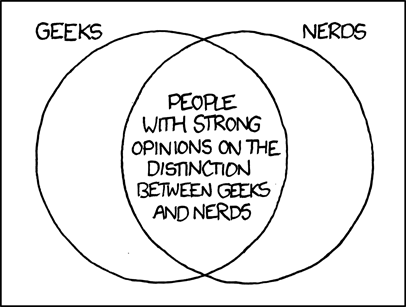
\includegraphics[width=\linewidth]{geeks_and_nerds.png}
\end{figure}

\newpage
\begin{figure}
\vspace{3cm}
\centering
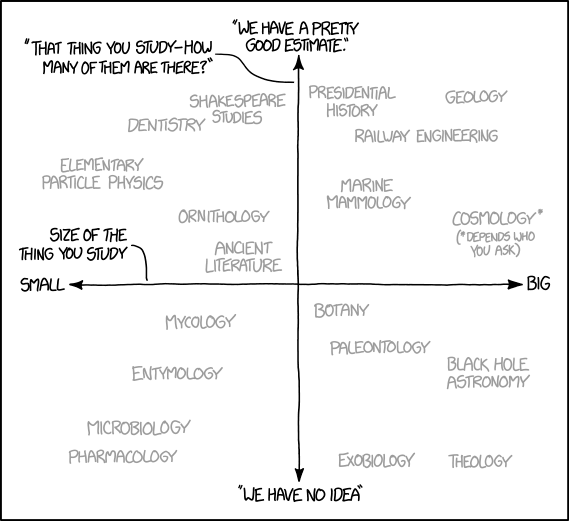
\includegraphics[width=\textwidth]{research_areas.png}

\end{figure}